\newpage
\subsubsection{Creating EReferences with MOSL}
\texHeader
\hypertarget{static:references tex}{}

In MOSL, the declaration of an EReference is simple - you set each property according to the following syntax (specified in simple EBNF, if you know what that
is):

\syntax{ [ `<>' ] `->' role\_name `(' multiplicity `)' `:'  target\_type \\
\\
With:\\
role\_name := STRING \\
multiplicity := `0..1' $|$ `0..*' $|$ `1' $|$ \ldots \\
target\_type := STRING \\
}

The source type is determined by the EClass in which the EReference is placed. You can signal an aggregation EReference by including the sideways diamond before
the arrow symbol. Don't worry - you don't have to remember this syntax. Our type completion provides a \texttt{reference} template when you activate the hot
keys. Try it out!

\begin{itemize}

\item[$\blacktriangleright$] Open \texttt{Box.eclass} in the editor and add a \emph{container reference} named \texttt{containedPartition} with a
multiplicity of zero to infinity, from \texttt{Box} to \texttt{Partition} (Fig.~\ref{eclipse:cpartitionReference}). This EReference means a \texttt{Box}
can hold an infinite number of partitions.

\vspace{0.5cm}

\begin{figure}[htbp]
	\centering
  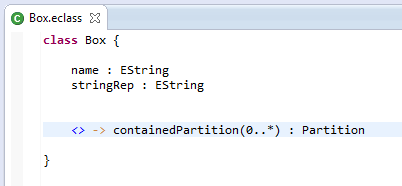
\includegraphics[width=0.6\textwidth]{eclass_box}
	\caption{Creating a \emph{container reference} in \texttt{Box}}
	\label{eclipse:cpartitionReference}
\end{figure} 

\vspace{0.5cm}

\item[$\blacktriangleright$] Now add a \emph{simple reference} to \texttt{Partition}. Name it \texttt{box}, and allow it to hold up to one \texttt{Box}
(Fig.~\ref{fig:boxReference}). This means a single partition can belong to either zero, or one \texttt{Box}, and that's it. It can't belong to two different
boxes at the same time.

\item[$\blacktriangleright$] Congratulations, you have just built your first pair of EReferences! To see how this is depicted visually, check out
Fig.~\ref{ea:ereference_completed} from the previous subsection.

\newpage

\vspace{0.5cm}

\begin{figure}[htbp]
	\centering
  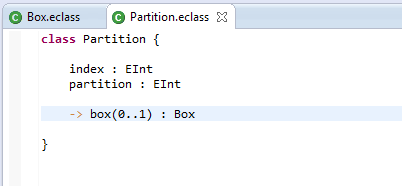
\includegraphics[width=0.6\textwidth]{eclass_partition}
	\caption{Creating a \emph{simple reference} in \texttt{Partition}}
	\label{fig:boxReference}
\end{figure} 

\vspace{0.5cm}

\item[$\blacktriangleright$] Now, lets create another pair of EReferences between \texttt{Partition} and \texttt{Card}. If you think about it, it's really not
all that different from the relation between \texttt{Box} and \texttt{Partition}. A \texttt{Partition} should be able to hold an unlimited amount of
\texttt{Card}s, but a \texttt{Card} should only be allowed to belong to zero or one \texttt{Partition}s. Name the two new EReferences
\texttt{card}, and \texttt{cardContainer}. Your EClasses should now closely resemble Fig.~\ref{eclipse:almostAllReferences}.

\begin{figure}[htbp]
	\centering
  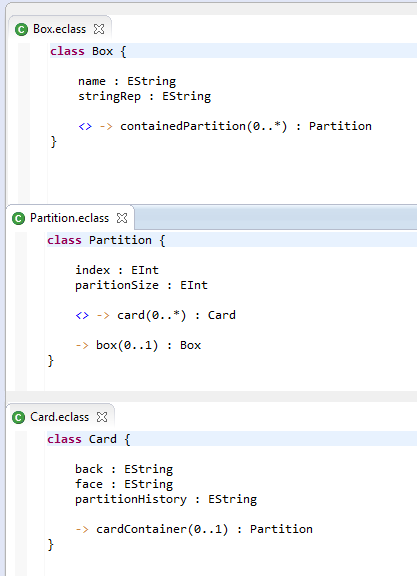
\includegraphics[width=0.58\textwidth]{eclipse_workspaceReferences}
	\caption{Completed EReference pairs}
	\label{eclipse:almostAllReferences}
\end{figure} 

\newpage

\item[$\blacktriangleright$] The next step is to construct two connections between \texttt{Partition}s so cards can be moved between their previous and next
partitions in the box. Create two new simple references, named \texttt{previous}, and \texttt{next}, each with a \texttt{0..1} multiplicity.

\vspace{0.5cm}

\item[$\blacktriangleright$] If you have done everything correctly, your EClasses should now resemble Fig.~\ref{eclipse:allReferences}. 

\vspace{0.5cm}

\begin{figure}[htbp]
	\centering
  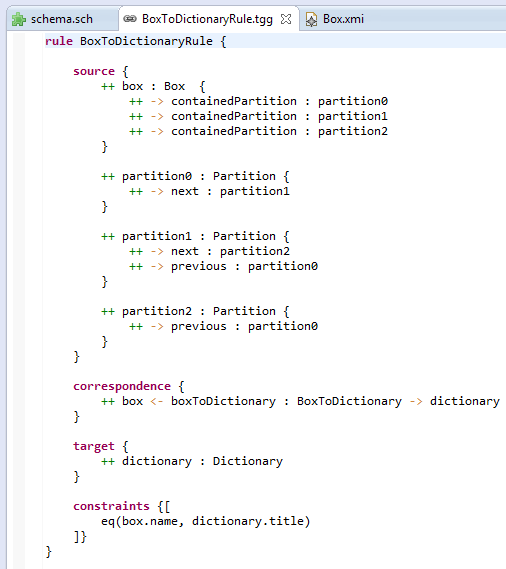
\includegraphics[width=0.6\textwidth]{eclipse_allReferences}
	\caption{All EReferences for Leitner's learning box}
	\label{eclipse:allReferences}
\end{figure} 

\clearpage

At this point, all of your EReferences have been created! The problem is, suppose you set the \texttt{containedPartition} EReference in a particular
\texttt{Box}. That's great, you would now have the box containing one partition. However, if you went and examined that partition independently, its
\texttt{box} EReference would still be null. We still need to set up the link between these EReferences so that when one is updated, the other will be too.

\vspace{0.5cm}

\item[$\blacktriangleright$] Navigate to the \texttt{\_constraints.mconf} file. You can see it has a single \texttt{opposites} scope that's currently empty.
Constraints follow the syntax below: 

\syntax{reference `<->' reference \\
\\
With:\\
reference := reference\_name `:' source\_type \\
reference\_name := STRING \\
source\_type := STRING \\}

This statement sets the two EReferences to be opposites of one another, i.e., the connection between EClasses will be bidirectional. As you can see, syntax here
is slightly different than that of a standard EReference. Instead of the reference type trailing the colon operator, it has switched to become the source type.

\vspace{0.5cm}

\item[$\blacktriangleright$] To begin, press \texttt{ctrl + space} and complete the template with the following:

\syntax{containedPartition : Box <-> box : Partition}

\item[$\blacktriangleright$] Reviewing the \texttt{Partition} EClass, its easy to see that \texttt{previous} and \texttt{next} are certainly not
opposites,\footnote{Review the rules depicted in Fig.~\ref{fig:membox_illustration}} but we do need to establish an opposing link between
\texttt{card} and its \texttt{cardContainer}. Follow the same steps until your constraint file resembles Fig.~\ref{eclipse:bothConstraints}.

\begin{figure}[htbp]
	\centering
  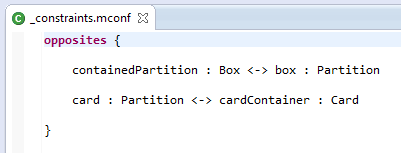
\includegraphics[width=0.6\textwidth]{eclipse_workspaceBothConstraints}
	\caption{The completed constraints file}
	\label{eclipse:bothConstraints}
\end{figure} 

\newpage

\item[$\blacktriangleright$] Now the EReferences for your learning box are complete! To see how each of the classes, attributes, and references
are depicted in the visual syntax, check out Fig.~\ref{ea:ereferences_all} from \hyperlink{sec:static vis}{section 2.1}. Otherwise, build your project to
make sure there are no errors, and continue to the next section to finalize the declaration of your EClasses.

\jumpSingle{static:methods tex}

\end{itemize}
